% Keep IEEEtran's original font encoding with both pdfLaTeX and XeTeX.
\RequirePackage[OT1]{fontenc}
\documentclass[conference,a4paper]{IEEEtran}

%%%%%%% Fill this out:
\newcommand{\trtitle}{Symbolic Planning for a Mobile Companion Robot: Action Costs}
\newcommand{\titleshort}{Mobile Companion Robot: Action Costs} % title for header:
\newcommand{\authorlastnames}{Gigar, Hooser} % alphabetical for seminars
\newcommand{\trcourse}{Knowledge Processing in Intelligent Systems: Practical Seminar}
\newcommand{\trsemester}{Winter Semester 2026/27}
\newcommand{\trgroup}{Knowledge Technology, WTM}
\newcommand{\truniversity}{Department of Informatics, Universit\"at Hamburg}
%%%%%%%%%%%%%%%%%%%%%%%%%%%%%%%%%%%%%%%%%%%%%%%%%%%%%%%%%%%%%
% Languages:

% If the thesis is written in English:
\usepackage[english]{babel}
\selectlanguage{english}

%%%%%%%%%%%%%%%%%%%%%%%%%%%%%%%%%%%%%%%%%%%%%%%%%%%%%%%%%%%%%
% Bind packages:

\usepackage{acronym}                    % Acronyms
\usepackage{algorithmic}				% Algorithms and Pseudocode
\usepackage{algorithm}				% Algorithms and Pseudocode
\usepackage{amsfonts}                   % AMS Math Packet (Fonts)
\usepackage{amsmath}                    % AMS Math Packet
\usepackage{amssymb}                    % Additional mathematical symbols
\usepackage{amsthm}
\usepackage{booktabs}                   % Nicer tables
%\usepackage[font=small,labelfont=bf]{caption} % Numbered captions for figures
\usepackage{color}                      % Enables defining of colors via \definecolor
\definecolor{uhhRed}{RGB}{254,0,0}		  % Official Uni Hamburg Red
\definecolor{uhhGrey}{RGB}{122,122,120} % Official Uni Hamburg Grey
\usepackage{fancybox}                   % Gleichungen einrahmen
\usepackage{fancyhdr}					% Packet for nicer headers
%\usepackage{fancyheadings}             % Nicer numbering of headlines

%\usepackage[outer=3.35cm]{geometry} 	  % Type area (size, margins...) !!!Release version
%\usepackage[outer=2.5cm]{geometry} 		% Type area (size, margins...) !!!Print version
%\usepackage{geometry} 					% Type area (size, margins...) !!!Proofread version
\usepackage{geometry} 	  % Type area (size, margins...) !!!Draft version
\geometry{a4paper,body={7.0in,9.1in}}

\usepackage{graphicx}                   % Inclusion of graphics
%\usepackage{latexsym}                  % Special symbols
\usepackage{longtable}				% Allow tables over several parges
\usepackage{listings}                   % Nicer source code listings
\usepackage{multicol}					% Content of a table over several columns
\usepackage{multirow}					% Content of a table over several rows
\usepackage{rotating}					% Alows to rotate text and objects
\usepackage[hang]{subfigure}            % Allows to use multiple (partial) figures in a fig
%\usepackage[font=footnotesize,labelfont=rm]{subfig}	% Pictures in a floating environment
\usepackage{tabularx}					% Tables with fixed width but variable rows
\usepackage{url,xspace,boxedminipage}   % Accurate display of URLs

%%%%%%%%%%%%%%%%%%%%%%%%%%%%%%%%%%%%%%%%%%%%%%%%%%%%%%%%%%%%%
% Configurationen:

\hyphenation{whe-ther} 				% Manually use: "\-" in a word: Staats\-ver\-trag

%\lstloadlanguages{C}                   % Set the default language for listings
\DeclareGraphicsExtensions{.pdf,.svg,.jpg,.png,.eps} % first try pdf, then eps, png and jpg
\graphicspath{{./src/}} 				% Path to a folder where all pictures are located
\pagestyle{fancy} 					% Use nicer header and footer

% Redefine the environments for floating objects:
\setcounter{topnumber}{3}
\setcounter{bottomnumber}{2}
\setcounter{totalnumber}{4}
\renewcommand{\topfraction}{0.9} 			  %Standard: 0.7
\renewcommand{\bottomfraction}{0.5}		  %Standard: 0.3
\renewcommand{\textfraction}{0.1}		  	%Standard: 0.2
\renewcommand{\floatpagefraction}{0.8} 	%Standard: 0.5

% Tables with a nicer padding:
\renewcommand{\arraystretch}{1.2}

%%%%%%%%%%%%%%%%%%%%%%%%%%%%
% Additional 'theorem' and 'definition' blocks:
\theoremstyle{plain}
\newtheorem{theorem}{Theorem}[section]
%\newtheorem{theorem}{Satz}[section]		% Wenn in Deutsch geschrieben wird.
\newtheorem{axiom}{Axiom}[section]
%\newtheorem{axiom}{Fakt}[chapter]		% Wenn in Deutsch geschrieben wird.
%Usage:%\begin{axiom}[optional description]%Main part%\end{fakt}

\theoremstyle{definition}
\newtheorem{definition}{Definition}[section]

%Additional types of axioms:
\newtheorem{lemma}[axiom]{Lemma}
\newtheorem{observation}[axiom]{Observation}

%Additional types of definitions:
\theoremstyle{remark}
%\newtheorem{remark}[definition]{Bemerkung} % Wenn in Deutsch geschrieben wird.
\newtheorem{remark}[definition]{Remark}

%%%%%%%%%%%%%%%%%%%%%%%%%%%%
% Provides TODOs within the margin:
\newcommand{\TODO}[1]{\marginpar{\emph{\small{{\bf TODO: } #1}}}}

%%%%%%%%%%%%%%%%%%%%%%%%%%%%
% Abbreviations and mathematical symbols
\newcommand{\modd}{\text{ mod }}
\newcommand{\RS}{\mathbb{R}}
\newcommand{\NS}{\mathbb{N}}
\newcommand{\ZS}{\mathbb{Z}}
\newcommand{\dnormal}{\mathit{N}}
\newcommand{\duniform}{\mathit{U}}

\newcommand{\erdos}{Erd\H{o}s}
\newcommand{\renyi}{-R\'{e}nyi}
\usepackage{graphicx}

% correct bad hyphenation here
\hyphenation{}

%%%%%%%%%%%%%%%%%%%%%%%%%%%%%%%%%%%%%%%%%%%%%%%%%%%%%%%%%%%%%
% Document:
\begin{document}

% Team 1 - Action Costs. Seminar instructor: Dr. Cornelius Weber.
\title{\trtitle\\[1.5ex]
\large \trcourse\\[0.5ex]
\trsemester\\[0.5ex]
\trgroup\\[0.5ex]
\truniversity}

\renewcommand{\headheight}{14.5pt}
\fancyhead[LO]{\slshape \authorlastnames}
\fancyhead[RO]{\slshape \titleshort}

\author{\IEEEauthorblockN{Saminas Hagos Gigar}
\IEEEauthorblockA{\textit{saminas.gigar@studium.uni-hamburg.de}}
\and
\IEEEauthorblockN{Alexandra Hooser}
\IEEEauthorblockA{\textit{alexandra.hooser@studium.uni-hamburg.de}}
}

\maketitle
\thispagestyle{fancy}

\begin{abstract}
A mobile companion robot can reach a goal in few actions and still incur a high execution cost. We investigate how minimizing weighted action cost changes plan length and modeled execution cost relative to minimizing action count. We model a building and a companion robot in the Planning Domain Definition Language (PDDL) and solve five paired navigation and delivery scenarios with Fast Downward 26.6 using A* with the landmark-cut heuristic. Both plans in each pair are evaluated using the same movement, door-opening, and manipulation costs. Across 30 runs, weighted-cost planning reduced total weighted action cost in four of five scenarios by 16.67\% to 50\%. The lower-cost plans used one or two additional actions. Both objectives achieved the same cost in the remaining scenario. The differences reflect route choice, reuse of an opened door, and the order in which objects are collected.
\end{abstract}

\IEEEpeerreviewmaketitle

\section{Introduction}
\label{sec:introduction}
A mobile companion robot fetching objects for a person must choose where to go, what to collect, and when to deliver it. Consider a closed service door between the entrance and a storage room. Opening it and moving directly to storage takes two actions. Moving around it takes four. If the door is costly to open and the corridors along the detour are cheap to traverse, counting actions favors the shortcut even though the modeled effort favors the detour. The decision changes again when the robot needs to return and can reuse the opened door.

We ask the following research question. \emph{How does minimizing total action costs influence plan length and travel cost compared to minimizing the number of actions in a simulated mobile robot environment?} We hypothesize that, in environments with different travel costs between rooms, cost-based planning will sometimes generate plans with more actions but lower total travel costs than action-count-based planning. Movement-only tasks directly illustrate that hypothesis. Door and delivery tasks extend the comparison to the total weighted action cost, which also includes opening and manipulation.

We evaluate an existing optimal planner on five paired tasks. We quantify the differences in plan length, modeled cost, and search effort and examine how changing the objective affects routes, door use, and collection order.

\section{Background and Related Work}
\label{sec:background}
Classical symbolic planning describes an initial state, actions with conditions and effects, and a goal. In the STRIPS tradition, actions transform a description of the world by adding and deleting facts. A plan is a sequence whose actions are applicable in order and whose final state satisfies the goal~\cite{fikes1971strips}. The Planning Domain Definition Language (PDDL) separates reusable action schemas and predicates in a domain file from the objects, initial facts, and goal of each problem. PDDL2.1 extends the language with numerical fluents and metrics for evaluating plans~\cite{fox2003pddl21}. Here we use the restricted action-cost fragment supported by Fast Downward~\cite{fd26pddl}.

Fast Downward translates PDDL into a finite-domain representation and searches forward through states~\cite{helmert2006fastdownward}. The landmark-cut heuristic, LM-cut, lower-bounds the remaining cost by identifying cuts of actions that every solution must cross in a relaxed task and accounting for their costs~\cite{helmert2009lmcut}. A* orders states by the sum of the cost already incurred and this lower bound. The admissible heuristic and Fast Downward's reopening of closed states support optimal search under the supplied nonnegative action costs~\cite{fd26eval,fd26astar}.

Symbolic task planning provides high-level choices that can be passed to execution systems. ROSPlan, for instance, integrates PDDL planning with action dispatch and feedback in ROS~\cite{cashmore2015rosplan}. Integrated task and motion planning also considers whether discrete action choices admit feasible continuous motions~\cite{garrett2021tamp}. Our evaluation concerns discrete plans over room transitions and object-handling actions. Planimation and the project's local player visualize symbolic state transitions for demonstrations. The evaluation uses planner outputs and a cost model, with no physical execution or ROS integration.

\section{Methodology}
\label{sec:methodology}
\subsection{Robot Environment and PDDL Model}
The five-room environment contains an entrance, hallway, office, meeting room, and laboratory. From the entrance the robot can reach the meeting room through the laboratory or through the hallway and office. The eight-room environment adds a library, classroom, and storage room. The hallway connects to storage through the library and classroom, and the meeting room also connects to storage. Each ordinary link in the tested problems is represented by two directed \texttt{connected} facts. The movement model can assign a separate cost to each direction.

Both domain variants use typed symbols for rooms, items, grippers, tables, people, doors, and cabinets. The robot occupies one room at a time. \texttt{move} requires that the robot be at the origin and that a directed connection to the destination exist. It deletes the old location and adds the new one. The service door is represented by \texttt{door-between} and \texttt{door-closed}. In door tasks the entrance--storage edge is initially absent. \texttt{open-door} requires a closed door with the specified endpoints and the robot at the origin endpoint. It removes the closed fact and adds both movement directions. The domain has no closing action, so the connection persists.

A pickup requires the robot and item to be in the same room and the selected gripper to be free. It replaces the item's room fact and the gripper's free fact with a \texttt{holding} fact. Placement on a co-located table and handover to a co-located person release the gripper and record \texttt{on-table} or \texttt{delivered-to}, respectively. Cabinet retrieval requires a co-located open cabinet, the item inside, and a free gripper. For the retrieval tasks the left and right grippers are distinct objects. Each can hold one item because pickup or cabinet retrieval consumes its free fact, and release restores it. The five benchmark scenarios exercise movement, door opening, pickup, and handover. Table placement and cabinet operations belong to the implemented domain and are outside this comparison.

\subsection{Action-Cost Modeling}
For a plan $\pi=(a_1,\ldots,a_n)$, the two objective functions are
\begin{align}
 C_{\mathrm{unit}}(\pi) &= \sum_{i=1}^{n} 1 = n, \\
 C_{\mathrm{w}}(\pi) &= \sum_{i=1}^{n} c_{\mathrm{w}}(a_i).
\end{align}
For movement from room $r$ to $s$, $c_{\mathrm{w}}$ is the assigned \texttt{distance}$(r,s)$. For opening door $d$, it is the assigned \texttt{door-opening-cost}$(d)$. Pickup, table placement, handover, cabinet opening, and cabinet retrieval each cost one. The assignments are synthetic, dimensionless units for comparing plans. They were chosen to distinguish the alternatives in these environments and have no physical calibration.

The cost domain declares \texttt{:action-costs} and uses \texttt{:functions} for the accumulator \texttt{total-cost} and the two static cost functions. Each problem initializes the accumulator to zero. Every action uses an \texttt{increase} effect to add its cost, and the problem metric is
\begin{center}
\texttt{(:metric minimize (total-cost))}.
\end{center}
Only the accumulator is updated. Applicability depends on logical facts. This follows Fast Downward's restriction to nonnegative integer action costs and at most one unconditional update of the total cost per action~\cite{fd26pddl}.

\subsection{Controlled Planner Comparison}
For each scenario the benchmark uses the same domain file and two problem files with the same objects, initial logical facts, and goal. The unit-cost version sets the static movement and door costs to one. The weighted-cost version changes those assignments while retaining the same feasible plan space. We use Fast Downward 26.6 with \texttt{astar(lmcut())} for both. The respective objectives yield a minimum-action plan and a minimum-weighted-cost plan. When minimum-action plans tie, the baseline is whichever plan Fast Downward returns. The experiment does not optimize weighted cost among those ties.

The benchmark reads the actions of each returned plan and applies the weighted problem's cost assignments to both plans. This common scoring rule makes the plans from both objectives comparable. The runner also checks that the unit planner's cost matches its action count and that the weighted planner's cost agrees with the recomputed weighted cost.

\section{Experimental Evaluation}
\label{sec:evaluation}
\begin{figure*}[t]
\centering
\subfigure[Total weighted action cost for both planning objectives.]{%
  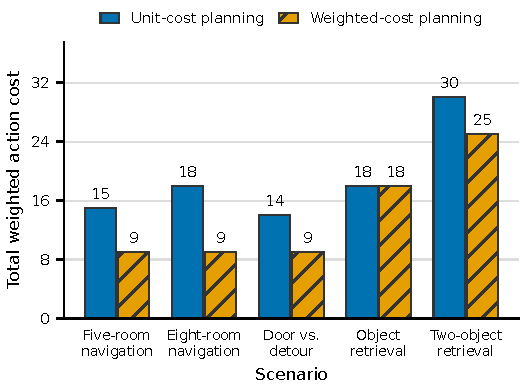
\includegraphics[width=0.49\textwidth]{weighted_cost_comparison}
  \label{fig:cost}}
\hfill
\subfigure[Number of actions in the plan.]{%
  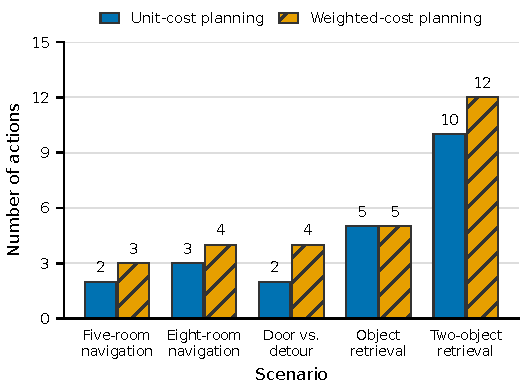
\includegraphics[width=0.49\textwidth]{plan_length_comparison}
  \label{fig:length}}
\caption{Median results over three repetitions per objective and scenario. The two series show plans obtained by minimizing action count and weighted action cost.}
\label{fig:comparison}
\end{figure*}

\subsection{Protocol and Metrics}
The navigation tasks start at the entrance and end in the meeting room (five rooms) or storage (eight rooms). The door-versus-detour task adds the closed service door to the eight-room instance. In single-object retrieval a book starts in storage and must reach the professor, who is at the entrance. Two-object retrieval additionally requires delivering a laptop from the office to the same recipient. Both retrieval tasks include the service door.

The saved evidence contains $5\times2\times3=30$ planner runs~\cite{kpisdata}. Each repetition ran the unit and weighted problems serially in that order, with a 60-second wall-clock limit per run and separate temporary working directories. All runs succeeded. The benchmark records plan length, evaluated weighted cost, and the number of expanded states reported by Fast Downward. Search time is the planner's reported search duration. Total runtime is measured around the planner process and includes translation and process overhead. The original machine configuration was not recorded in the benchmark log.

For each objective we report medians over its three repetitions. For repetition $j$, the percentage reduction in total weighted action cost is
\begin{equation}
 R_j=100\,
 \frac{C_{\mathrm{w}}(\pi_{\mathrm{unit},j})-
       C_{\mathrm{w}}(\pi_{\mathrm{w},j})}
      {C_{\mathrm{w}}(\pi_{\mathrm{unit},j})}\,\%.
\end{equation}
We report the median of the three paired reductions. All baselines in the evidence have positive weighted cost. Action-count differences are likewise computed within each pair. Within each objective and scenario, action counts, weighted costs, and expanded states were identical across repetitions.

\subsection{Observed Plans}
Figure~\ref{fig:comparison} shows that weighted optimization lowered cost in four tasks, with one or two more actions in each. Table~\ref{tab:effort} gives the percentage reductions and search effort.

In five-room navigation the minimum-action plan goes through the lab in two moves costing $8+7=15$. Weighted-cost planning chooses three moves through the hallway and office at a cost of $3+3+3=9$. The eight-room unit-cost plan continues from the meeting room to storage for a total of 18 units across three moves. Weighted-cost planning reaches storage through the hallway, library, and classroom for 9 units across four moves. These two tasks isolate the effect of the movement assignments.

For the door-versus-detour task, the two-action shortcut costs 12 to open and 2 to traverse. The weighted plan takes four moves at a cost of 9 and leaves the door closed. When fetching the book, both objectives instead use the door on the return trip as well as on the way out. Its one-time opening charge, two traversals, pickup, and handover sum to $12+2+2+1+1=18$. A door-free round trip also costs 18 in movement alone, so adding the two manipulation actions would cost 20. The persistent effect of opening the door changes the comparison between a one-way journey and a round trip.

For the two-object task, the minimum-action plan opens the door, picks up the book in storage, and collects the laptop in the office on the way back. Weighted-cost planning collects the laptop first, visits storage for the book, and returns through the classroom, library, and hallway. Both objects can be carried for the final part of the trip and handed over at the entrance. Avoiding the door lowers the cost from 30 to 25, while the number of actions rises from 10 to 12. This is the collection order in the observed plan. The experiment does not establish uniqueness among minimum-cost plans.

\begin{table}[t]
\caption{Median paired cost reduction and median states expanded per search. U and W denote the unit- and weighted-cost objectives.}
\label{tab:effort}
\centering
\begin{tabular}{@{}lrrr@{}}
\toprule
 & Cost reduction & \multicolumn{2}{c}{Expanded states} \\
\cmidrule(l){3-4}
Scenario & (\%) & U & W \\
\midrule
Five-room navigation & 40.00 & 3 & 4 \\
Eight-room navigation & 50.00 & 4 & 5 \\
Door vs. detour & 35.71 & 3 & 5 \\
Object retrieval & 0.00 & 6 & 8 \\
Two-object retrieval & 16.67 & 21 & 24 \\
\bottomrule
\end{tabular}
\end{table}

\section{Discussion and Limitations}
For the same feasible plan space, the returned minimum-action plan is also a candidate for weighted optimization. Consequently, the minimum weighted cost is at most the weighted cost of that baseline. The empirical question is how large the difference is and which decisions account for it. In both navigation cases, extra moves reduced movement cost. For door versus detour and two-object retrieval, movement cost rose by seven units (2 to 9 and 14 to 21, respectively). In both cases the 12-unit saving from avoiding the door outweighed the extra movement cost. Thus the weighted objective can trade higher movement cost for lower total weighted action cost. The single-object result shows why the one-time charge cannot be assessed from the outward leg alone. Whether it is worth paying depends on how the plan uses the resulting connection.

Weighted-cost planning expanded one to three more states in each measured task (Table~\ref{tab:effort}). Changing costs changes both A*'s path-cost ordering and the heuristic's estimates. These counts describe the particular searches and provide no general ranking of the objectives by search effort. Across scenario/objective medians, search times were about 0.040 to 0.267 ms and whole-process runtimes about 65 to 73 ms. The tasks complete too quickly for these few timings to give a meaningful runtime ranking. Repeating deterministic tasks measures repeatability on five instances and adds no independent scenarios. We therefore report descriptive results without significance tests.

The environments are small, designed by hand, and use synthetic costs. A different choice of movement or door costs could change the preferred plan. The minimum-action tie-breaking also affects the size of the measured benefit. There was no independent VAL validation. The symbolic model assumes deterministic transitions, with no continuous paths, collision checks, perception uncertainty, dynamic obstacles, or execution failures. It was not deployed on a physical robot. The results concern modeled action cost and cannot quantify real-world savings. Larger task sets, systematic variation of the cost assignments, calibration from measured executions, and independent plan and physical execution checks would test how well these patterns transfer.

\section{Conclusion}
The observations support the hypothesis on the two navigation tasks. Weighted-cost planning chose longer routes on cheaper links. Across all five tasks, it lowered total weighted action cost in four cases, with a maximum reduction of 50\%, and tied the minimum-action solution in single-object retrieval. The door and delivery cases show how a persistent change to the environment and the sequence of pickups can affect that trade-off. The additional state expansions describe these small instances.

\section*{Acknowledgments and Use of Tools and AI}
Fast Downward produced the plans, and Python and Matplotlib summarized and plotted the benchmark measurements~\cite{kpisdata}. OpenAI Codex assisted with software development, analysis, literature searches and reference checks, drafting, and LaTeX preparation. The authors are responsible for verifying the evidence, claims, and references and for revising and approving the final paper.

% Keep long repository and documentation URLs readable in a narrow column.
\begingroup
\raggedright
\bibliographystyle{plain}
\bibliography{bib}
\endgroup
\end{document}
